

%\documentclass[pra,twocolumn,epsfig,rotate,superscriptaddress,showpacs]{revtex4}


% \mathcal{u}se only LaTeX2e, calling the article.cls class and 12-point type.

\documentclass[prl,twocolumn,showpacs]{revtex4-1}
\usepackage{graphicx}
\usepackage{epsfig}
\usepackage{epsf}
\usepackage{amssymb}
\usepackage{amsmath}
\usepackage{amsthm}
\usepackage{multirow}
\usepackage{hyperref}

% \renewcommand{\familydefault}{\sfdefault}  %% arial font
% \usepackage{times} %% times new roman font

\newcommand{\bra}[1]{\langle #1|}
\newcommand{\ket}[1]{|#1\rangle}

\newcommand{\be}{\begin{equation}}
\newcommand{\ee}{\end{equation}}
\newcommand{\bea}{\begin{eqnarray}}
\newcommand{\eea}{\end{eqnarray}}
\newcommand{\Fig}[1]{Fig.\,\ref{#1}}
\newcommand{\Eq}[1]{Eq.\,(\ref{#1})}
\newcommand{\la}{\langle}
\newcommand{\ra}{\rangle}
\newcommand{\nl}{\nonumber \\}
\usepackage[usenames]{color}
\definecolor{Red}{rgb}{1,0,0}
\definecolor{Blue}{rgb}{0,0,1}






%%%%%%%%%%%%%%%%% END OF PREAMBLE %%%%%%%%%%%%%%%%



\begin{document}

% Include your paper's title here
\title{Experimental Estimation of Average Fidelity of a Clifford Gate on a 7-qubit Quantum Processor}
\author{Dawei Lu$^{1}$}
\author{Hang Li$^{1,2}$}
\author{Denis-Alexandre Trottier$^{1}$}
\author{Jun Li$^{1,3}$}
\author{Aharon Brodutch$^{1}$}
\author{Jonathan Baugh$^{1,4}$}
\author{Raymond Laflamme$^{1,5}$}
\email{laflamme@iqc.ca}


\affiliation{$^{1}$Institute for Quantum Computing and Department of Physics,
University of Waterloo, Waterloo N2L 3G1, Ontario, Canada}
\affiliation{$^{2}$Department of Physics, Tsinghua University, Beijing, 100084, China}
\affiliation{$^{3}$Department of Modern Physics, University of Science
and Technology of China, Hefei, Anhui, 230026, China}
\affiliation{$^{4}$Department of Chemistry, University of Waterloo, Waterloo N2L 3G1,
Ontario, Canada}
\affiliation{$^{5}$Perimeter Institute for Theoretical Physics, Waterloo, Ontario,
Canada}


\begin{abstract}
The traditional approach of characterizing a quantum gate via quantum process tomography requires exponential number of experiments, and hence makes the average fidelity estimation of a specific quantum gate impractical even for moderately large systems. In this paper, we certified a nontrivial Clifford gate in a 7-qubit nuclear magnetic resonance (NMR) system efficiently through adopting the twirling protocol and sampling method simultaneously. We obtained that the average fidelity of this Clifford gate is about 0.55, and rises to 0.87 after eliminating the decoherence effect. The experimental spectrum of the pseudo-pure state based on the implementation of this Clifford gate is also shown, from which we can state that reliable coherent controls have been achieved in our system. The entire protocol of certifying Clifford gates is efficient and scalable, as well as easily extended to other systems with minor modifications.
\end{abstract}
\pacs{03.67.Lx, 07.57.Pt, 42.50.Dv, 76.60.-k}

\maketitle



\paragraph*{Introduction.}

The methodology in characterizing the level of coherent control is fundamental and important in evaluating potential quantum information processing (QIP) devices. It can provide a fair and intuitionistic comparison of controlling abilities between diverse QIP devices and also indicate the prospects of a designated system with respect to fault-tolerant quantum computation. The traditional characterizing approach quantum process tomography (QPT) is able to realize complete characterization of a quantum channel, and has been applied to utmost 3-qubit systems in experiment. However, QPT suffers the exponentially growing resources with the number of qubits, which leads to the impracticality of its implementation even in relatively small systems. Moreover, in many cases full knowledge of a particular quantum gate by QPT is not necessary because some other physical descriptions of the gate are sufficient to reveal the noise level and require much less experiments than QPT.  Several methods such as randomized benchmarking, twirling, Monte Carlo estimations have been proposed to evaluate a particular quantum channel in an efficient manner, while all of them have their own restrictions and drawbacks. Here, in order to benchmark our coherent control on a 7-qubit nuclear magnetic resonance (NMR) system, we adopted the twirling protocol to estimate the average fidelity of an important Clifford gate in QIP. The gate we certified enables the generation of the maximal order coherence from single coherence with the aid of merely local rotations, which is indispensable for preparing the cat state in multi-qubit systems. The estimation method is scalable and independent of number of qubits, as well as easily implemented in experiments. From the results and experimental spectra we have shown that reliable coherent control have been achieved in our system.

\paragraph*{Theory.}

When a desired unitary operator $\mathcal{U}$ is applied in experiment, the real operator $\tilde{\mathcal{U}}$ will involve a noisy part $\Lambda$ $\tilde{\mathcal{U}} = \Lambda \circ \mathcal{U}$. The average fidelity $\bar{F}(\mathcal{U}, \tilde{\mathcal{U}})$ between $\mathcal{U}$ and $\tilde{\mathcal{U}}$ is defined as
\begin{align} \label{average_fidelity}
\bar{F}(\mathcal{U}, \tilde{\mathcal{U}}) &= \int d\mu(\psi) \bra{\psi} \mathcal{U}^{\dagger}\circ \tilde{\mathcal{U}} (\ket{\psi} \bra{\psi}) \ket{\psi} \\
&= \int d\mu(\psi) \bra{\psi} \mathcal{U}^{\dagger}\circ \Lambda \circ \mathcal{U} (\ket{\psi} \bra{\psi}) \ket{\psi},
\end{align}
where $d\mu(\psi)$ is the unitarily invariant distribution of pure states known as Fubini-Study measure\cite{Emerson2005}. Since a random state can be generated from a fixed state by applying a random unitary, we can equivalently average over a distribution of random unitaries invariant under conjugation
\begin{align} \label{average_Harr}
\bar{F}(\mathcal{U}, \tilde{\mathcal{U}}) &= \int d\mu(V) \bra{\psi} V^{\dagger} \mathcal{U}^{\dagger}\circ \Lambda \circ \mathcal{U} V(\ket{\psi} \bra{\psi}) \ket{\psi},
\end{align}
where $d\mu(V)$ is a unitarily invariant distribution of random unitaries known as Harr measure\cite{Emerson2005}.

%\begin{figure}[htb]
%\begin{center}
%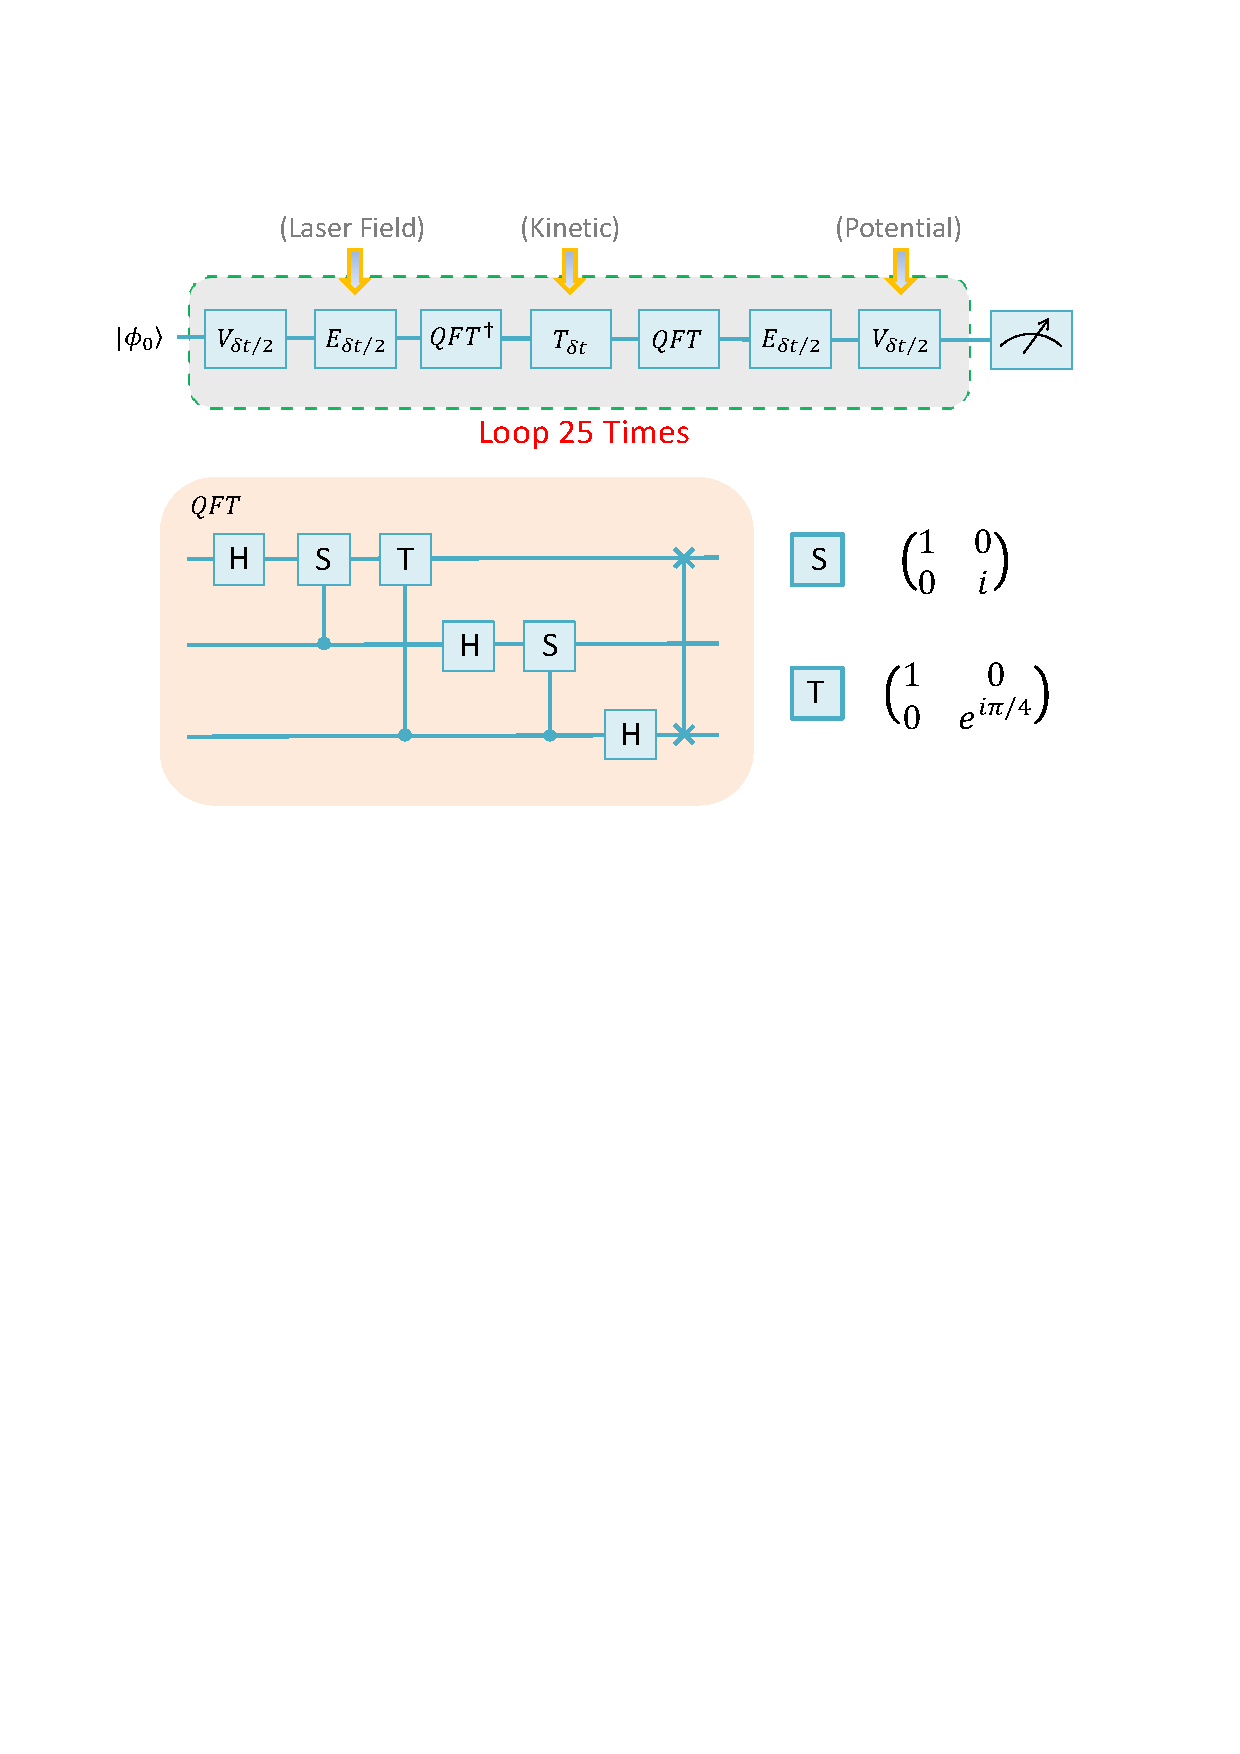
\includegraphics[width=\columnwidth]{circuit.pdf}
%\end{center}
%\setlength{\abovecaptionskip}{-0.35cm}
%\caption{\footnotesize{(color online). Circuit for twirling procedure based on the Clifford group $\mathcal{C}$. $\tilde{\mathcal{U}} = \Lambda \circ \mathcal{U}$ is the superoperator to describe the desired unitary $\mathcal{U}$ associated with some noise $\Lambda$. $M_\psi$ and $M_{\psi, \mathcal{C}_i, \mathcal{U}}$ are the original and modified measurement operators, respectively. In this protocol $\text{P}_1, \text{P}_2$ and $\text{P}_3$ are all Pauli operators and can be computed efficiently.}}\label{circuit}
%\end{figure}

After twirled with such Harr-distributed unitaries, a quantum channel will be reduced to a depolarizing channel, with the noise strength and average fidelity described by a single parameter\cite{Emerson2007}. However, it requires exponential number of  elementary gates to create a random Harr-distributed unitary, which makes the estimation of average fidelity inefficient based on Harr measure. Fortunately, a unitary 2-design\cite{Dankert2009} is proved to be able to obtain an analytical expression of Eq. \ref{average_Harr}, by replacing the integral with a sum over the finite group. In particular, the Clifford group $\mathcal{C}$ is one example of unitary 2-designs, thus Eq. \ref{average_Harr} can be written as
\begin{align} \label{average_Clifford}
\bar{F}(\mathcal{U}, \tilde{\mathcal{U}}) &= \frac{1}{|\mathcal{C}|}\sum_i \bra{\psi} \mathcal{C}_i^{\dagger} \mathcal{U}^{\dagger}\circ \Lambda \circ \mathcal{U} \mathcal{C}_i(\ket{\psi} \bra{\psi}) \ket{\psi}.
\end{align}
In other words, averaging over $\mathcal{C}$ and averaging over Harr measure lead to the same average fidelity.

The relevant circuit of this twirling procedure by the Clifford group is depicted in Fig. \ref{everything}(a). $\mathcal{C}_i$ is a local randomized Clifford operation, $\tilde{\mathcal{U}} = \Lambda \circ \mathcal{U}$ is a faulty unitary gate we want to certify, $M_\psi$ is the original measurement operator related to $\ket{\psi}$, and $M_{\psi, \mathcal{C}_i, \mathcal{U}} = \mathcal{U}\mathcal{C}_i M_\psi \mathcal{C}_i^{\dagger}\mathcal{U}^{\dagger}$ is the modified measurement operator by combining the last three components in the circuit. Note that if the initial state P$_1$ is a Pauli operator and the desired unitary gate $\mathcal{U}$ belongs to the Clifford group, then $\text{P}_2 = \mathcal{C}_i \text{P}_1 \mathcal{C}_i^{\dagger}$ and $\text{P}_3 = M_{\psi, \mathcal{C}_i, \mathcal{U}}= \mathcal{U}\mathcal{C}_i \text{P}_1 \mathcal{C}_i^{\dagger}\mathcal{U}^{\dagger}$ are also Pauli operators. This is due to the fact that Clifford propagators cannot transform Pauli operators out of the Pauli group. The remained signal $S_i$ after this simulated depolarizing channel will be
\begin{align} \label{remain_signal}
S_i = \text{Tr} \left( \tilde{\mathcal{U}} \left(\mathcal{C}_i\text{P}_1\mathcal{C}_i^{\dagger} \right) \text{P}_3\right) = \text{Tr} \left( \tilde{\mathcal{U}} \left( \text{P}_2\right) \text{P}_3\right).
\end{align}
Here, $\tilde{\mathcal{U}}(\rho)$ denotes the density matrix by applying the superoperator $\tilde{\mathcal{U}}$ on $\rho$.

There are two reasons that we merely consider a Clifford gate $\mathcal{U}$ and corresponding Pauli operators in this protocol. First, for a general unitary gate, it is impractical to realize the modified measurement operator $M_{\psi, \mathcal{C}_i, \mathcal{U}}$ in an efficient manner. Whereas for a Clifford gate and original Pauli measurement $M_\psi$,  $M_{\psi, \mathcal{C}_i, \mathcal{U}}$ can be calculated efficiently\cite{Aaronson2004}. Second, The Clifford group gates construct elementary units in majority of fault-tolerant quantum computations based on stabilizer codes, and the universality is granted via magic state preparation\cite{Bravyi2005}. For instance, the encoding operation of the 3-qubit quantum error correction code is a Clifford gate comprising two controlled-NOT (CNOT) gates and a  single qubit Hadamard gate, and has been certified in a 3-qubit solid-state NMR system\cite{Moussa2012}.

For a $n$-qubit system, the average fidelity of a faulty Clifford gate $\tilde{\mathcal{U}} = \Lambda \circ \mathcal{U}$ is\cite{Alex2013}
\begin{align} \label{final_fidelity}
\bar{F}(\mathcal{U}, \tilde{\mathcal{U}}) = \frac{1}{M}\sum_{i=1}^{M} S_i= \frac{1}{M}\sum_{i=1}^{M}\text{Tr}\left( \tilde{\mathcal{U}} \left( \mathcal{P}_i\right) \mathcal{P}_{k_i}\right),
\end{align}
which is the natural extension of Eq. \ref{remain_signal}.  $M = 4^n-1$ is the number of elements in $n$-qubit Pauli group, $\mathcal{P}_i$ is the Pauli state after applying $\mathcal{C}_i$, and $\mathcal{P}_{k_i} = \mathcal{U} \mathcal{P}_i \mathcal{U}^{\dagger}$ is the corresponding Pauli observable.  The meaning of Eq. \ref{final_fidelity} is let $\text{P}_2$ in Eq. \ref{remain_signal} span over the entire Pauli group $\mathcal{P}$, which has $M = 4^n-1$ elements, and calculate the average remained signal. If $\tilde{\mathcal{U}}$ is perfect, i.e. $\tilde{\mathcal{U}} = \mathcal{U}$, obviously $\bar{F} =1$ which is consistent.

In spite of the tractability of Eq. \ref{final_fidelity} to estimate the average fidelity of Clifford gates, the complexity remains exponential as $4^n-1$ different Pauli states need to be prepared and thus the same number of expectation values have to be determined.  However, in principle measuring all of the expectation values is unnecessary if one only desires to approximate the mean. The Hoeffding's inequality\cite{Venkatesh2012} states that if $x_1, . . . ,x_m$ are independent realizations of
a random variable $X$, confined to the interval $[a, b]$ and with statistical mean $\mathbb{E}(X) = \mu$, then for any $\delta >0$ we have
\begin{align} \label{Hoeffding}
\text{P} \left( |\bar{X}-\mu| > \delta \right) \leq 2e^{-2\delta^2N/(b-a)^2},
\end{align}
where $\bar{X} = \frac{1}{N}\sum_{i=1}^m x_i$ is the estimator of the exact mean $\mu$, and $\text{P}(\epsilon)$ denotes the probability of event $\epsilon$. The Hoeffding's inequality provides an upper bound to the probability that the estimated mean is off by a value greater than $\delta$.

Back to our task of estimating the average fidelity by Eq. \ref{final_fidelity}, it is reasonable to set $a=0$ and $b=1$ as the bound of expectation values. Hence, for a given $\text{P}$ and $\delta$, the number of experiments for Eq. \ref{final_fidelity} is
\begin{align} \label{exp_number}
m\leq \frac{\text{ln}(2/\text{P})}{2\delta^2}
\end{align}
by taking natural logarithm of each side of Eq. \ref{Hoeffding}. Note that the number of experiments is independent of number of qubit $n$, once the desired accuracy $\text{P}$ and precision $\delta$ have been given. This result shows that the twirling protocol is efficient and scalable with the number of qubits increasing. For instance, given a $99\%$ accuracy and 0.04 precision, the total number of experiments is 1656, regardless of whatever number of qubits in the system.

\begin{figure*}[htb]
\begin{center}
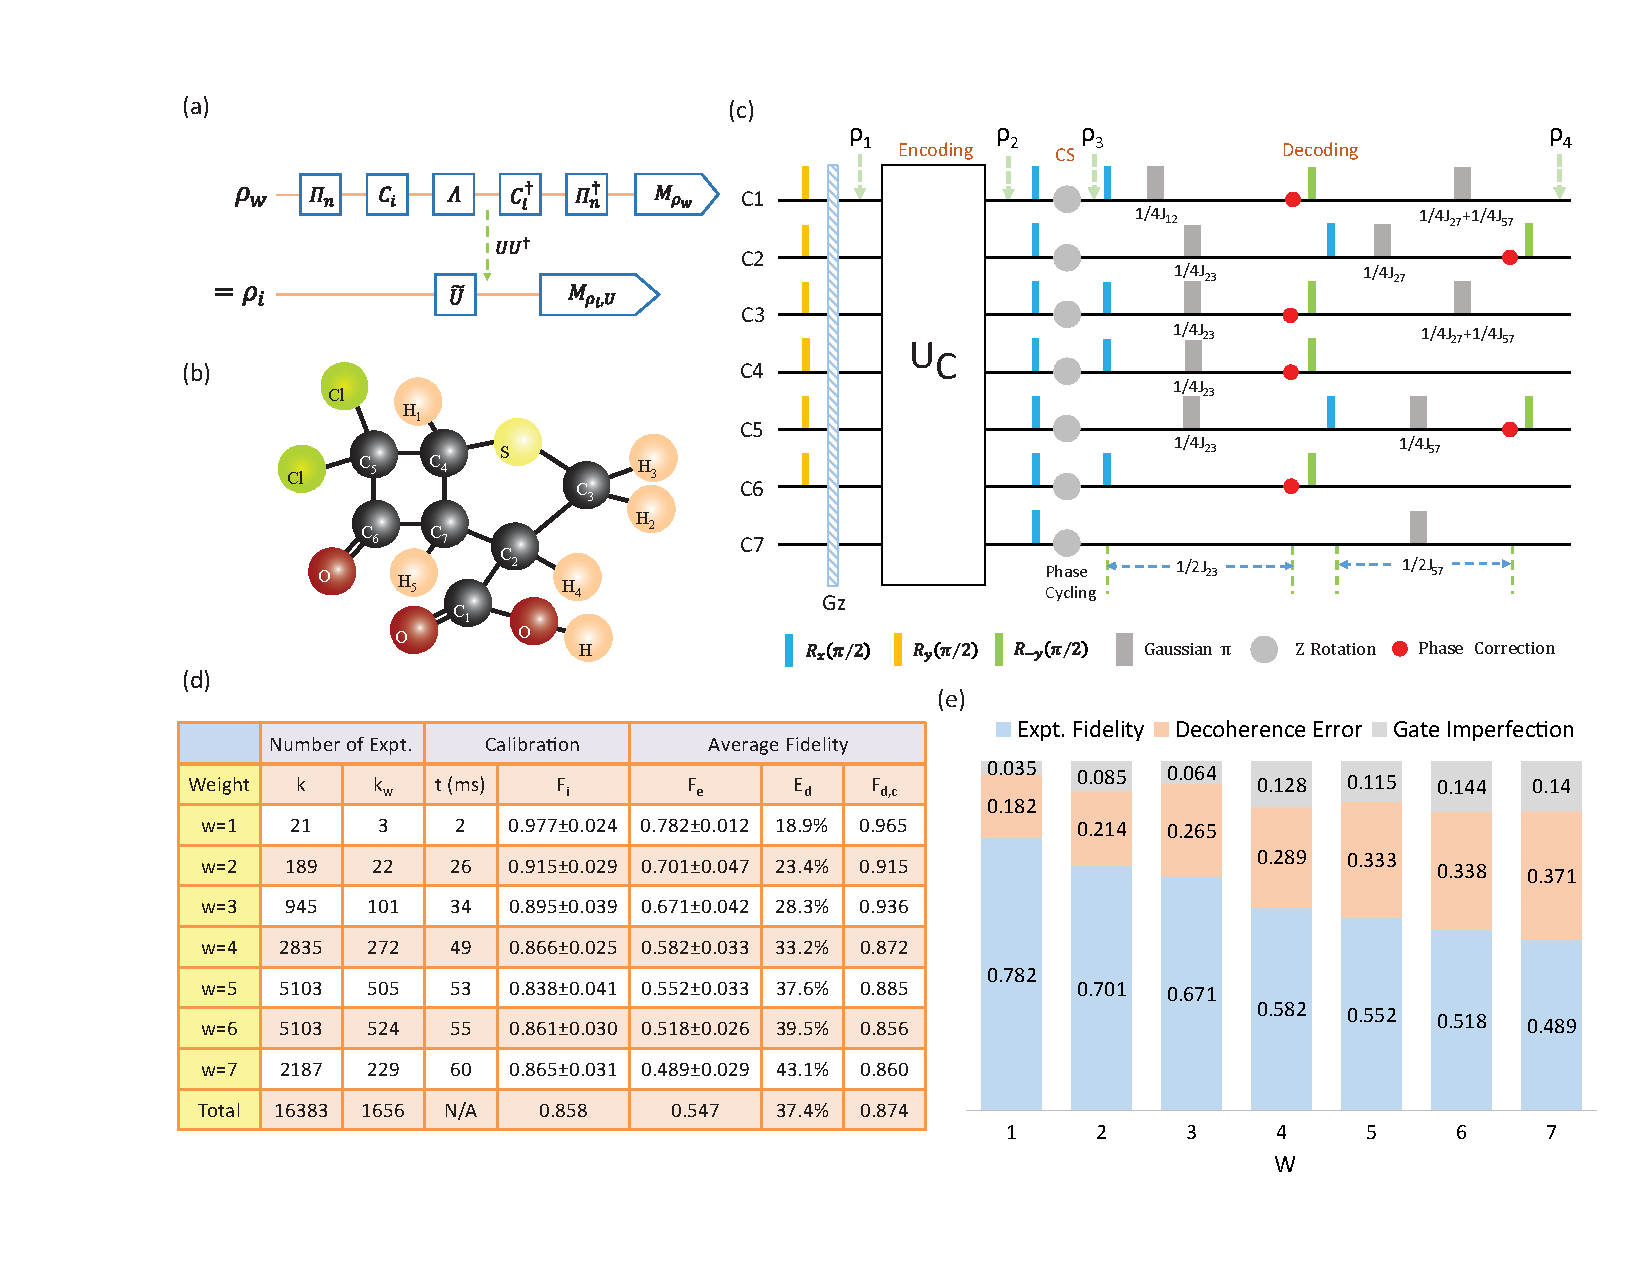
\includegraphics[width=2\columnwidth]{everything2.pdf}
\end{center}
\setlength{\abovecaptionskip}{-0.35cm}
\caption{\footnotesize{(color online). (a) Circuit for twirling procedure based on the Clifford group $\mathcal{C}$. $\tilde{\mathcal{U}} = \Lambda \circ \mathcal{U}$ is the superoperator to describe the desired unitary $\mathcal{U}$ associated with some noise $\Lambda$. $M_\psi$ and $M_{\psi, \mathcal{C}_i, \mathcal{U}}$ are the original and modified measurement operators, respectively. In this protocol $\text{P}_1, \text{P}_2$ and $\text{P}_3$ are all Pauli operators and can be computed efficiently. (b) Molecular structure of Dichloro-cyclobutanone, where C$_1$ to C$_7$ form a 7-qubit system. (c) Pulse sequence for the creation of labeled PPS via the method in Ref. \cite{Knill2000}. It consists of three parts: encoding, coherence selection (CS) and decoding. $\mathcal{U}_{C}$, realized by a 80ms GRAPE pulse, is the Clifford gate to be certified. The instantaneous states are (unnormalized) $\rho_1 = \sigma^7_z$,  $\rho_2 = \sigma^1_z\sigma^2_z\cdots \sigma^7_z$, $\rho_3 = \ket{00\cdots 0}\bra{00\cdots 0}+\ket{11\cdots 1}\bra{11\cdots 1}$, and $\rho_4 =  \ket{00\cdots 0}\bra{00\cdots 0} \bigotimes \sigma^7_z$, respectively. (d) Experimental result for the certification of $\mathcal{U}_{C}$. $k$ is the number of Pauli operators for a designated weight $w$, while $k_w$ is the number of experiments via the sampling; $t$ is the typical time for the input Pauli state preparation, and $F_i$ is the calibration to capture the errors in preparation and measurement; $F_e$ is the experimental result of the probability of no error, and $F_{d,c}$ is the same quantity but without decoherence effect $E_d$. (e) Relationship among the experimental average fidelities (blue), decoherence effects (orange) and gate imperfections (gray) for different $w$.}}\label{everything}
\end{figure*}

\paragraph*{Experiment.}
The Clifford gate $\mathcal{U}_{C}$ to certify in our experiment was chosen as the main-body operator in generating maximal coherence from single coherence. It evolves $ZI\cdots I$ to $ZZ\cdots Z$, and thus indispensable for the pseudo-pure state (PPS) preparation via the method proposed in Ref. \cite{Knill2000}, as the role of encoding process ($\mathcal{U}_{C}$ in Fig. \ref{everything}(c)). Besides, it also serves as the essential component for the creation of cat state $\left( \ket{00\cdots 0}+\ket{11\cdots 1} \right)/\sqrt{2}$ up to a certain number of phase gates. In NMR, it can be decomposed into a chain of elementary Clifford gates
\begin{align} \label{decomp}
e^{-i\frac{\pi}{2}I_x^i}e^{-i\pi I_z^i I_z^j} e^{-i\frac{\pi}{2}I_y^i},
\end{align}
which can improve the order of coherence by evolving $Z_i$ to $Z_i Z_j$, with $I_x^i$ being spin-1/2 operator and so forth. Moreover, implementing this Clifford gate in experiment, e.g. in NMR, is nontrivial as it requires $2(n-1)$ single qubit operations and $n-1$ 2-qubit operations, even without counting the refocusing gates inserted in the interaction. Therefore, estimating the average fidelity of the aforementioned Clifford gate in experiment is not only significant from QIP point of view, but also well-representative to evaluate the level of coherent controls in a given quantum device.

Our 7-qubit sample is $^{13}$C labeled Dichloro-cyclobutanone dissolved in d6-acetone. The structure of the molecule is shown in Fig. \ref{everything}(b), where we denote C$_1$ to C$_7$ as our seven qubits. $^1$H nuclei were decoupled by standard Waltz-16 sequence throughout all the experiments. The internal Hamiltonian of this system can be described as 
\begin{align}\label{Hamiltonian}
\mathcal{H}_{int}=&&\sum\limits_{j=1}^7 {2\pi \nu _j } I_z^j  + \sum\limits_{j < k,=1}^7 {2\pi} J_{jk} I_z^j I_z^k,
\end{align}
where $\nu_j$ is the resonance frequency of the \emph{j}th spin and $\emph{J}_{jk}$ is the scalar coupling strength between spins \emph{j} and \emph{k}. See supplemental material for the values of all parameters. All experiments were conducted on a Bruker DRX 700MHz spectrometer at room temperature.

The entire procedure to estimate the average fidelity of $\mathcal{U}_{C}$ can be divided into four parts, and the details are as follows.

(i) Sampling. To achieve a given accuracy 99\% and precision 0.04, we obtained that the required number of experiments is 1656 via Eq. \ref{exp_number}, which is indeed independent of number of qubits. Next we randomly sampled 1656 Pauli states out of the entire 7-qubit Pauli group, which has in total $4^7-1=16383$ elements. We divided all of the selected experiments to seven subgroups according to the weight of each Pauli state, where the weight of a Pauli operator is defined as the number of non identity terms in its tensor product form. The primary reason for this division is that an arbitrary gate such as $\mathcal{U}_{C}$ is often more vulnerable when applied on a highly weighted Pauli state. Thus the signal loss of Eq. \ref{remain_signal} depends on the weights of initial Pauli states. 

The sampling result is shown in Fig. \ref{everything}(d), where the number of sampled experiments $k_w$ for weight $w$ is around one tenth of the number of all Pauli operators with weight $w$. 

(ii) Preparation and Calibration. For the creation of every sampled initial Pauli state, we employed the sequence compiling program\cite{Ryan2008} to produce a scalable pulse sequence. All the pulses appeared in the preparation sequences are local, while generated by Gaussian shapes. Then we calibrated the results aiming to capture the errors in preparation and measurements. The typical duration $t$ for preparing a weight $w$ Pauli state and the related calibrations $F_i$ are both listed in Fig. \ref{everything}(d).

(iii) Evolution. Our target operation $\mathcal{U}_{C}$ was realized by the GRadient Ascent Pulse Engineering (GRAPE) pulse\cite{Khaneja2005}, based on the pulse sequence for the encoding procedure as an initial guess. Utilizing GRAPE algorithm is able to guarantee that $\mathcal{U}_{C}$ belongs to the Clifford group, as traditional shape pulses and sequences for multiple qubits in NMR are usually hard to make a Clifford operation due to the large amount of strongly state-dependence and simplification. The GRAPE pulse of $\mathcal{U}_{C}$ was obtained with the pulse width chosen as 80ms and a theoretical fidelity 0.99, and then rectified in experiment to minimize the discrepancies between the ideal and real pulses\cite{Weinstein2004}.

(iv) Measurement. After applying the GRAPE pulse of $\mathcal{U}_{C}$ to any initial Pauli state in experiment, we measured the corresponding final Pauli state by local pulses, and recorded the signal loss.  Next we averaged the results and calculated the fidelity $F_e$ with respect to different weight $w$, as shown in Fig. \ref{everything}(d). It is reasonable that the average fidelity decreases substantially with $w$ increasing, as 
high order coherent terms are extremely fragile to the decoherence occurred during $\mathcal{U}_{C}$. 

The column $F_e$ in Fig. \ref{everything}(d) illustrates that the probability of no error is 54.7\%, meaning the average fidelity of $\mathcal{U}_{C}$ is about 55.1\% according to Eq. \ref{xxxxxxxxxx}. Considering that  $\mathcal{U}_{C}$ roughly comprises twelve 1-qubit gates and six 2-qubit gates, the average error per gate $\simeq 2.5\%$. To assess the decoherence effect in $\mathcal{U}_{C}$, we followed the approach of phase damping \cite{Vandersypen2001} to simulate the dynamical process step by step. The average signal attenuation due to decoherence is shown in the column $E_d$ in Fig. \ref{everything}(d). Under the assumption that the decoherence error is factorable, the probability of no error after eliminating the decoherence is 87.4\%. Hence, compared to 55.1\% with decoherence, the average fidelity without decoherence rises to 87.5\%. The average error per gate $\simeq 0.7\%$, which is mainly attributed to the imperfection in the design and implementation of the GRAPE pulse.  Fig. \ref{everything}(e) displays straightforwardly the relationship among the experimental average fidelities, decoherence effects and gate imperfections for different $w$. 

We also showed the spectrum of $\sigma^1_z\sigma^2_z\cdots \sigma^7_z$ as the expected result of $\mathcal{U}_{C} \sigma^7_z \mathcal{U}_{C}^{\dagger}$ with the observation of C$_2$ in Fig. XXXXX. From the comparison between the simulated and experimental spectra, it convinces us reliable coherent control has been achieved in this 7-qubit system, in spite of inevitable decoherence.  Moreover, we continued to prepare the labeled PPS based upon the network in Fig. \ref{everything}(c), which employs $\mathcal{U}_{C}$ as the encoding procedure. The PPS spectrum by observing the labeled spin C$_7$ is shown in Fig. XXXXX.

\paragraph*{Conclusion.}
In conclusion, we have shown how to efficiently estimate the average fidelity of a Clifford gate using a twirling protocol and random sampling. 

\begin{thebibliography}{99}
\bibitem{Moussa2012} O. Moussa, M. da Silva, C. Ryan, and R. Laflamme, Phys. Rev. Lett. \textbf{109}, 070504 (2012).
\bibitem{Emerson2005} J. Emerson, R. Alicki, and K. Zyczkowski, J. Opt. B \textbf{7}, S347 (2005).
\bibitem{Emerson2007} J. Emerson \emph{et al.}, Science \textbf{317}, 1893 (2007).
\bibitem{Dankert2009} C. Dankert, R. Cleve, J. Emerson, and E. Livine, Phys. Rev. A \textbf{80}, 012304 (2009).
\bibitem{Aaronson2004} S. Aaronson and D. Gottesman, Phys. Rev. A \textbf{70}, 052328 (2004).
\bibitem{Bravyi2005} S. Bravyi and A. Kitaev, Phys. Rev. A \textbf{71}, 022316 (2005).
\bibitem{Alex2013} D. Trottier, Master thesis, University of Waterloo, 2013.
\bibitem{Venkatesh2012} S. Venkatesh, \emph{The Theory of Probability: Explorations and Applications}. Cambridge University Press, 2012.
\bibitem{Knill2000} E. Knill, R. Laflamme, R. Martinez, C. Tseng, Nature \textbf{404}, 368 (2000).
\bibitem{Ryan2008} C. Ryan \emph{et al.}, Phys. Rev. A \textbf{78}, 012328 (2000).
\bibitem{Khaneja2005} N. Khaneja \emph{et al.}, J. Magn. Reson. \textbf{172}, 296 (2005).
\bibitem{Weinstein2004} Y. Weinstein \emph{et al.}, J. Chem. Phys. \textbf{121}, 6117 (2005).
\bibitem{Vandersypen2001} L. Vandersypen \emph{et al.}, Nature \textbf{414}, 883 (2001).
\end{thebibliography}


\end{document}
